\documentclass[12pt,a4paper]{article}
\usepackage[utf8]{inputenc}
\usepackage[margin=1in]{geometry}
\usepackage{graphicx}
\usepackage{amsmath}
\usepackage{amsfonts}
\usepackage{enumerate}
\usepackage{listings}
\usepackage{xcolor}
\usepackage{float}
\usepackage{booktabs}
\usepackage{calc}
\usepackage{tikz}
\usetikzlibrary{positioning, arrows.meta, shapes.geometric}

\definecolor{codegreen}{rgb}{0,0.6,0}
\definecolor{codegray}{rgb}{0.4,0.4,0.4}
\definecolor{codepurple}{rgb}{0.58,0,0.82}
\definecolor{backcolour}{rgb}{0.95,0.95,0.92}

\lstdefinestyle{mystyle}{
    backgroundcolor=\color{backcolour},   
    commentstyle=\color{codegreen},
    keywordstyle=\color{blue},
    numberstyle=\tiny\color{codegray},
    stringstyle=\color{codepurple},
    basicstyle=\sffamily\footnotesize,
    breakatwhitespace=false,         
    breaklines=true,                 
    captionpos=b,                    
    keepspaces=true,                 
    numbers=left,                    
    numbersep=5pt,                  
    showspaces=false,                
    showstringspaces=false,
    showtabs=false,                  
    tabsize=4
}

\lstset{style=mystyle}

% Title and Author
\title{Auto-reproducability literature review}
\author{Andreas Moe}
\date{\today}

\begin{document}

\maketitle

\section{Abstract}

\section{Introduction}
\subsection{Rationale}
\subsection{Objectives}
\section{Methods}
\subsection{Eligibility criteria}
\subsection{Information sources}
\subsection{Search strategy}
\subsection{Selection process}
\subsection{Data collection process}
\subsection{Data items}
\subsection{Study risk of bias assessment}
\subsection{Effect measures}
\subsection{Synthesis methods}
\subsection{Reporting bias assessment}
\subsection{Certainty assessment}
\section{Results}
\subsection{Study selection}
\newpage

\begin{figure}[H]
\centering
\resizebox{\textwidth}{!}{%
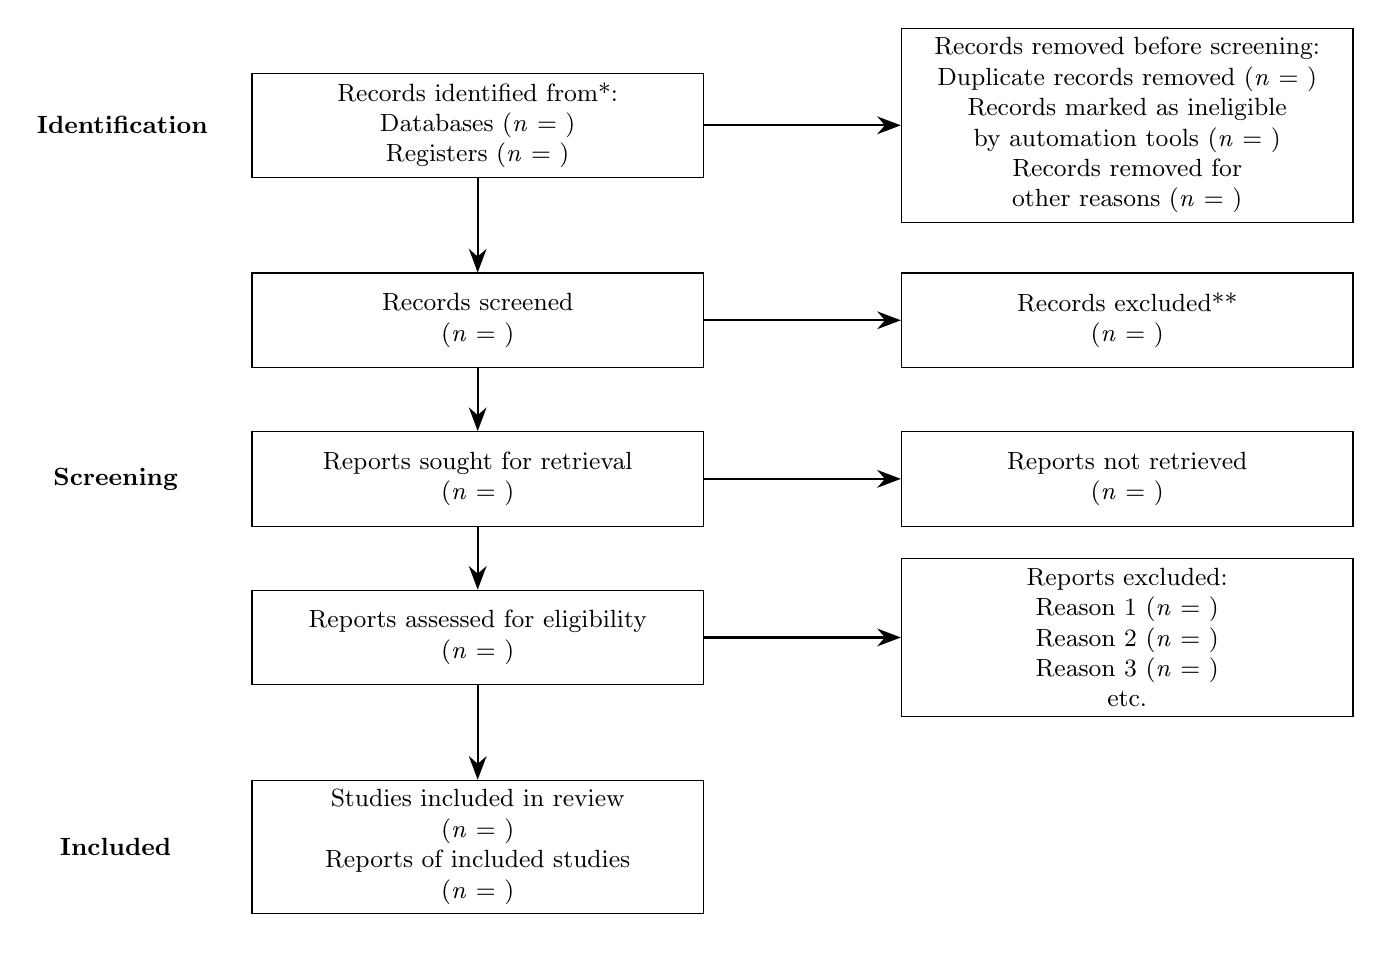
\begin{tikzpicture}[
    node distance=0.8cm and 1.5cm,
    box/.style={rectangle, draw, text width=5.5cm, minimum height=1.2cm, align=center, font=\small},
    label/.style={rectangle, text width=2cm, align=center, font=\small\bfseries, minimum height=2.2cm},
    arrow/.style={-{Stealth[length=3mm]}, thick},
]
\node[box] (identified) {Records identified from*:\\ Databases (\textit{n} = )\\ Registers (\textit{n} = )};
\node[box, right=2.5cm of identified] (removed) {Records removed before screening:\\ Duplicate records removed (\textit{n} = )\\ Records marked as ineligible\\ by automation tools (\textit{n} = )\\ Records removed for\\ other reasons (\textit{n} = )};
\node[box, below=1.2cm of identified] (screened) {Records screened\\ (\textit{n} = )};
\node[box, right=2.5cm of screened] (excluded1) {Records excluded**\\ (\textit{n} = )};
\node[box, below=0.8cm of screened] (sought) {Reports sought for retrieval\\ (\textit{n} = )};
\node[box, right=2.5cm of sought] (notretrieved) {Reports not retrieved\\ (\textit{n} = )};
\node[box, below=0.8cm of sought] (assessed) {Reports assessed for eligibility\\ (\textit{n} = )};
\node[box, right=2.5cm of assessed] (excludedreasons) {Reports excluded:\\ Reason 1 (\textit{n} = )\\ Reason 2 (\textit{n} = )\\ Reason 3 (\textit{n} = )\\ etc.};
\node[box, below=1.2cm of assessed] (included) {Studies included in review\\ (\textit{n} = )\\ Reports of included studies\\ (\textit{n} = )};
\node[label, left=0.6cm of identified] (idlabel) {Identification};
\node[label, left=0.6cm of sought, minimum height=4.5cm] (scrlabel) {Screening};
\node[label, left=0.6cm of included] (inclabel) {Included};
\draw[arrow] (identified) -- (screened);
\draw[arrow] (identified) -- (removed);
\draw[arrow] (screened) -- (excluded1);
\draw[arrow] (screened) -- (sought);
\draw[arrow] (sought) -- (notretrieved);
\draw[arrow] (sought) -- (assessed);
\draw[arrow] (assessed) -- (excludedreasons);
\draw[arrow] (assessed) -- (included);

\end{tikzpicture}%
}
\caption{PRISMA 2020 flow diagram for new systematic reviews which included searches of databases and registers only. Source: Page MJ, et al. BMJ 2021;372:n71. doi: 10.1136/bmj.n71. Licensed under CC BY 4.0.}
\label{fig:prisma}
\end{figure}

\noindent\footnotesize{*Consider, if feasible to do so, reporting the number of records identified from each database or register searched (rather than the total number across all databases/registers).}\\
\noindent\footnotesize{**If automation tools were used, indicate how many records were excluded by a human and how many were excluded by automation tools.}
\normalsize
\subsection{Study characteristics}
\subsection{Risk of bias in studies}
\subsection{Results of individual studies}
\subsection{Results of syntheses}
\subsection{Reporting biases}
\subsection{Certainty of evidence}
\section{Discussion}
\subsection{Interpretation}
\subsection{Limitation of evidence}
\subsection{Limitaion of review processes}
\subsection{Implications}
\section{Other information}

\newpage
\begin{appendix}
\section*{Appendix}

\end{appendix}


\begin{thebibliography}{1}

% \bibitem{}

\end{thebibliography}


\end{document}